% 1982 年全国卷（理科）第 7 题：空间四边形 ABCD 及各边中点 M、N、P、Q（按源卷布局）。
% A 在左、B 在上、C 在下、D 在右；M(AB)、N(BC)、P(CD)、Q(DA) 依次连成四边形 MNPQ。
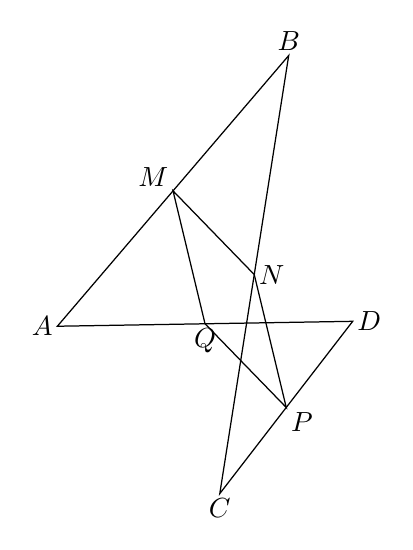
\begin{tikzpicture}[scale=1.25, line width=0.45pt,
  every node/.style={inner sep=1.5pt}]
  \coordinate (A) at (0,0);
  \coordinate (B) at (2.35,2.75);
  \coordinate (C) at (1.65,-1.70);
  \coordinate (D) at (3.00,0.05);
  \coordinate (M) at (1.175,1.375);   % AB 中点
  \coordinate (N) at (2.000,0.525);   % BC 中点
  \coordinate (P) at (2.325,-0.825);  % CD 中点
  \coordinate (Q) at (1.500,0.025);   % DA 中点
  % 空间四边形 ABCD
  \draw (A) -- (B) -- (C) -- (D) -- cycle;
  % 中点四边形 MNPQ
  \draw (M) -- (N) -- (P) -- (Q) -- cycle;
  \node[left] at (A) {$A$};
  \node[above] at (B) {$B$};
  \node[below] at (C) {$C$};
  \node[right] at (D) {$D$};
  \node[above left] at (M) {$M$};
  \node[right] at (N) {$N$};
  \node[below right] at (P) {$P$};
  \node[below] at (Q) {$Q$};
\end{tikzpicture}
